\documentclass{article}
\usepackage{geometry}
\usepackage{amsmath}
\usepackage{titling}
\usepackage{graphicx}
\usepackage{hyperref}

\hypersetup{colorlinks=true,urlcolor=cyan,linkcolor=blue}

\pretitle{\begin{center}\huge}
\posttitle{\end{center}}
\preauthor{\begin{center}\small}
\postauthor{\end{center}}
\predate{\begin{center}\footnotesize}
\postdate{\end{center}}
\setlength{\droptitle}{-40pt}

\title{Probe Scanning Circuit} 
\date{May, 2022}
\author{Brian Frost}
\begin{document}

\maketitle

\section{Introduction}

\par{The OCT scanning probe developed in our lab scans via the driving of a piezoelectric plate with a voltage waveform. We want to control the scanning of the probe We want using ThorImage, as well as our acquisition program which uses the ThorLabs SpectralRadar SDK. These methods are designed by ThorLabs with their hardware in mind, and are not directly compatible with our probe hardware.}
\par{In short, the probe scanning circuit acts as an adapter. We have access to the voltage waveform used to control the scanning mirrors, and we input this signal to our circuit to generate a waveform which equivalently scans the probe.}
\par{ThorImage and the SpectralRadar SDK allow the user to control the field of view over which they are scanning. We would like this value to match with the true field of view being scanned by the probe. We would also like to use the full possible scanning range of the probe allowed by the piezo driver -- a voltage amplifier at the very end of the circuit pipeline. We often refer to this driver as ``the blue box."}
\par{Lastly, we would like to be able to finely control the position of the probe at which M-Scans will be taken. That is, when the probe is not scanning, we would like to be able to carefully adjust its position so that we can measure a specific structure. This functionality of the scanning circuit is to be implemented entirely in hardware, rather than being controlled by ThorImage.}
\par{In this document, we will first describe the waveform output by the Telesto when it is scanning its mirrors, which acts as the \textit{input} to our circuit. We will then discuss the specifications necessary for the adaptation of this signal to our scanning probe, i.e. we will describe the \textit{output} of the circuit. Lastly, we will discuss the implementation of this circuit, and how it may be used with either ThorImage or our acquisition program.}

\section{The Input Waveform}

\par{The ThorLabs Telesto is equipped with two scanning mirrors, each of which is controlled by a separate voltage waveform. This allows for scanning at any angle, via controlling the behavior of both mirrors at once. Our scanning probe is equipped only with a single piezo, allowing scanning only along a single axis. As such, we will concern ourselves only with the voltage waveform for a single mirror. The center in $X$ and $Y$ of the B-Scan can also be set in ThorImage, which amounts to a DC offset on each mirror's control voltage.}
\par{When the scanning probe was first built by Nathan Lin, the signal for the Y mirror was used. When the angle in ThorImage or the SpectralRadar SDK is set to -90$^\circ$, the mirrors scan only in the Y direction and the field of view displayed on the screen is equivalent to the Y field of view. We have also designed the circuit to operate with center $(0,0)$, as we would like to control the offset ourselves (as described in the introduction, as well as in the following section).}
\subsection{Scanning Parameters}
\par{The sampling rate, $f_S$, describes the rate at which A-Scans are taken, not to be confused with the rate at which B-Scans are taken. Each B-Scan comprises a number of parallel A-Scans. Either the number of scans, $N$ or Y-pixel size, $\delta Y$, can be controlled. We can use these parameters to compute the rate at which B-Scans are taken $f_B$, either in terms of $N$ or $\delta Y$ and the field of view: 
	\begin{align}
		f_B &= \frac{f_S}{N}, \\
		f_B &= \frac{f_S\delta Y}{FOV}.
	\end{align}
The latter equation comes from the identity $N = FOV/\delta Y$. The Telesto III system has 5 in-built sampling rates: 10 kHz, 28 kHz, 48 kHz, 76 kHz and 146 kHz. It allows at maximum $N=10000$ A-Scans per B-Scan.}
\par{The probe configuration file contains parameters regarding what is (erroneously) referred to as the apodization process. In OCT processing, a background spectrum identical to the light source spectrum is used to normalize the recorded signal. In standard operation, this is recorded before each B-Scan via ``flying back" the mirrors into their ``apodization position." This is a position in which no light from the sample beam will be reflected to the photodetectors, so that only the reference beam (shaped like the source) will be recorded and used as the background in processing.}
\par{Our probe has no such position to fly back to, and we must measure the background in a different way. This will be the subject of a different document. For now, I will just say that it is important to set the following parameters in the config file to ensure that this flyback does not occur, and that an incorrect background is not used in ThorImage's processing:
\begin{itemize}
	\item{\texttt{SizeOfApodization=0} -- The total number of samples taken in the flyback position.}
	\item{\texttt{ApodizationCycles=0} -- The number of samples piced out from the \texttt{SizeOfApodization} total samples to be averaged to compute the background.}
	\item{\texttt{FlybackTime=0} -- The amount of time over which the mirror swings into position.}
	\item{\texttt{ApoVoltage=0,0} -- The voltage controlling the X and Y mirrors at the flyback position.}
\end{itemize}
These parameters are set in a file called \texttt{Probe0Spike.ini}.}
\subsection{Character of the Signal}
\par{With these parameters in mind, we can now describe the signal seen at the output of the Telesto, or the input of our circuit. The position of the mirror is controlled linearly by the voltage, with slope $m=-720$ mV/mm. Over the field of view $FOV$ centered at zero, this means that the voltage follows a ramp shape from $V_0=-mFOV/2$ to $-V_0$ over a period of $T_B = 1/f_B$. This ramp signal is $T_B$-periodic, repeating until scanning is stopped.}
\par{A general cartoon of this signal can be seen in Fig. \ref{input}. A specific example of this signal displayed on an oscilloscope with $FOV=1$ mm, $N=10000$ and $f_S = 146$ kHz is shown in Fig. \ref{inputscope}. In this case, the value of $m$ above gives $V_0 = 360$ mV (as this means a total 720 mV is swept). The period is $T_B = N/f_s = 10000/146000\approx68.5$ ms.}


\section{Specifications}
\par{We need the output of the circuit to adhere to a set of important specifications, due both to the nature of the piezo driving amplifier and the mechanical properties of the piezoelectric itself. We also want to ensure that the FOV value in ThorImage and the acquisition software match the FOV actually swept by the probe. We will cover these issues in turn.}
\subsection{Voltage Limit Specifications}
\par{The piezo driving amplifier has a linear voltage gain of 20, with maximum input voltage range of -9 V to +9V (corresponding to an output range of -180 V to +180 V). As stated before, we want to use the entire voltage range so that we can achieve the maximal FOV for the probe. However, we must be careful not to exceed these limits and risk breaking the driver. Thus, our voltage specification is that \textbf{the output voltage must never exceed 9 V in magnitude.}}
\subsection{Frequency Specifications -- Mechanical Ringing and Scanning Frequency}
\par{As can be seen in Fig. \ref{input}, the control voltage quickly jumps from $-V_0$ to $+V_0$ when a new B-Scan acquisition begins. This jump comprises many high frequency components, which can cause mechanical ringing in the piezoelectric at its resonant frequency. This is undesirable, as it creates a spatial oscillation at the left end of our B-Scan.}
\par{We need to remove this ringing by softening the jump, via application of a low-pass filter (LPF). The resonant frequency seems to vary between piezoelectric plates, so we determine the required LPF cutoff frequency $f_C$ emperically. Testing for several probes, we found a cutoff frequency of around 20 Hz to be sufficient to avoid ringing.}
\par{Note however that the main frequency coomponent of the signal is actually the frequency at which B-Scans are taken, $f_B = 1/T_B$. We do not want to significantly attenuate or phase-shift this frequency via our LPF. Thus, our frequency specification is \textbf{the output signal must be filtered by an LPF with cutoff frequency of 20 Hz, and the scanning frequency must be significantly lower than 20 Hz.}}
\subsection{Field of View Specifications}
\par{We want to achieve the maximal scanning FOV allowed by our piezo and driver. This is the FOV when the driver outputs its maximum voltage, -180 to +180. This is different for each piezoelectric plate as well, so we must determine this empirically for each probe. We measure this maximum FOV $FOV_{max}$ for each probe, and note that this corresponds to a scanning circuit output of -9V to +9V. This means that we want our circuit to output -9 V to +9 V when the ThorImage or acquisition program displays an FOV of $FOV_{max}$.}
\par{At $FOV_{max}$, say the mirror control signal at the circuit's input ranges from $-V_{max}$ to $+V_{max}$. This means that \textbf{the circuit must have a linear voltage gain of $\mathbf{9/V_{max}}$}. As $FOV_{max}$, and thereby $V_max$, will change between probes, this means that \textbf{the circuit must have a variable voltage gain}.}
\par{To provide a ballpark value for the voltage gain, we found that one probe has a maximum scanning range of $FOV_{max} =360$ $\mu$m. This corresponds to an input voltage of about $\pm 130$ mV, and thereby we need a gain of about $70$. This means that \textbf{the variable linear gain should be on the order of magnitude of 50-100}.}
\subsection{Input and Output Impedance}
\par{Two easy specifications to miss are the input and output impedances of our circuit, which control the possible current draw of the circuit given certain voltage values. The input impedance determines how much current will be drawn from the input, in this case the Telesto's mirror driver. As we do not know how much current this circuit is capable of producing, it is safest to make this impedance very large so that a small amount of current is drawn. The output impedance determines how much current can be drawn from the circuit at the output, in this case by the piezo driver. We want the piezo driver to ``get as much current as it needs," so a low output impedance is preferable here. That is, \textbf{we want our circuit to have a very high input impedance and very low output impedance.}}
\section{Implementation}
\par{According to the specifications described above, we have designed a circuit consisting of four stages -- a variable-gain amplifier, a variable-offset unity-gain summing amplifier, a low-pass filter and a unity gain buffer. To satisfy the voltage constraints, we also include +9 V and -9 V voltage regulators.}
\par{Fig. \ref{block} displays a block diagram for the circuit, including the form the signal will take at the output of each block. In order, the amplifying stage adjusts the voltage so that the FOV in ThorImage/the acquisition program matches that of the probe. The summing amplifier adds a variable DC voltage offset to the signal, so as to allow the user to control the position at which M-Scans are being taken. The LPF softens the jump between B-Scan acquisitions so as to reduce mechanical ringing. The unity gain buffer does not affect the voltage at all, but gives the circuit near-zero output impedance. Each block is described very briefly below.}


\subsection{Voltage Amplifier}

\par{The op amp circuit for a non-inverting voltage amplifier is shown in Fig. \ref{noninvamp}. The gain of this circuit is given by $A=1+\frac{R_2}{R_1}$, so 
	\begin{equation}
		V_{out} = V_{in}\Big(1+\frac{R_2}{R_1}\Big).
	\end{equation}
In our circuit, $V_in$ is the output of the Telesto. Replacing either of $R_1$ or $R_2$ with a potentiometer allows for a variable gain. In our case, we allow $R_2$ to vary}

\subsection{Summing Amplifier}

\par{The op amp circuit for a unity-gain summing amplifier is shown in Fig. \ref{summer}. The circuit yields the relationship
	\begin{equation}
		V_{out} = V_{in} + V_{DC}.
	\end{equation}
In our circuit, $V_{in}$ here is the output of the amplification stage, and $V_{DC}$ is the user-controlled offset. The offset is determined by placing a potentiometer between the rails, so that it acts as a voltage divider. The variable potentiometer output is $V_{DC}$, and can take any value between the rails (in our case $\pm 9$ V).}

\subsection{Low-Pass Filter}

\par{The op amp circuit for a first-order low-pass filter is shown in Fig. \ref{lpf}. It can be shown that the transfer function of this circuit is
	\begin{equation}
		\frac{V_{out}(\omega)}{V_{in}(\omega)} = \frac{e^{j\arctan{\omega RC}}}{\sqrt{1+R^2C^2\omega^2}}.
	\end{equation}
Both the amplitude and phase response here are of interest. As the frequency increases, the output magnitude decreases and the output phase varies more from the input phase.}
\par{The cutoff frequency $f_C$ is defined as the frequency at which the output is a factor of $\sqrt{2}$ smaller than the input in magnitude. In units Hz, this is
	\begin{equation}
		f_C = \frac{1}{2\pi RC}.
	\end{equation}
In our circuit, we want a cutoff frequency of around 20 Hz to attenuate the mechanical ringing of the piezo. However, it is not desirable to attenuate the B-Scan frequency or to incur a large phase shift between the input and output waveforms. This would result in a displayed B-Scan which is not spatially representative of the space over which the probe has swept in the same timeframe. This means that we would like $f_B$ to be small relative to $f_C$.}

\subsection{Unity Gain Buffer}

\par{The schematic for a unity-gain buffer is shown in Fig. \ref{buff}. The buffer has the same topology as the non-inverting amplifier, except with $R_1 = \infty$ and $R_2 = 0$. Thereby, the gain is $1+R_2/R_1 = 1$. The purpose of this circuit is to ensure a high output impedance.}

\subsection{The Complete Schematic and Value Choices}
\par{The completed schematic is shown in Fig. \ref{schem}. This fleshes out the block diagram into all of its parts as described above, and includes the regulating power circuitry above. The values of these parts are listed in Table \ref{materials}.}

\par{All discrete resistors are chosen to be 100 k$\Omega$ for convenience, as resistors of this value are very easy to find. The first potentiometer $RV_1$ is chosen to be 50 k$\Omega$. This yields a minimum gain of $1 + \frac{100000}{50000} = 3$ to $\infty$. The second potentiometer $RV_2$ acts as a variable voltage divider, and thereby could theoretically work at any value. A relatively large value of 500 k$\Omega$ is chosen because it will draw less current, which is safer with respect to overheating and over-drawing from the regulators.}
\par{The regulator datasheets suggest values of $C_{1-4}$ around 0.1 $\mu$F. We began with these values, then found that the $\pm$9 V power rails were still noisy. To reduce noise at the power rails, we included 0.47 $\mu$F capacitors in parallel between the rails and ground. This yields $C_{2,4}$ total capacitance values of 0.57 $\mu$F.}
\par{Finally, $C_5$ is chosen as 0.1 $\mu$F as it yields a cutoff frequency of $1/2\pi R_5C_5 \approx 16$ Hz.}

\subsection{Physical Inplementation}
\par{The interior and exterior of the box containing the circuit are shown in Figs \ref{inside} and \ref{outside}, respectively. The circuit itself is built of standalone IC regulators and DIP op-amps, soldered onto two Adafruit breadboards.}
\par{The DC offset control potentiometer is on the left side of the box, which the gain control is on the right side of the box. The input and output are labeled. The ON/OFF switch connects the $\pm$15 V power supply to the regulators, so the circuit draws no current if the switch is flipped off. It is thereby safe to leave the box plugged in. The box is grounded.}
\section{Application}
\par{Our chosen capacitance and resistance values gives a cutoff frequency of about 16 Hz. If we scan at $f_S=16$ Hz, with $N=10000$ A-Scans per B-Scan, then $f_B=2.8$ Hz. This is significantly lower than the cutoff and thereby the LPF does not incur a large phase shift.}
\par{Below, we show examples on an oscilloscope of the circuit operating with these parameters. The 2.8 Hz scanning frequency can be seen from the 250 ms/div time axis. In Fig. \ref{samplenormal}, we show the circuit in a usual operation mode. Here, the DC offset is set to about 0 and the gain is set to about 62.5. The output voltage range is smaller than $\pm9$ V, so no saturation occurs. The softening of the jump as a result of the LPF is visible. Note that the Telesto signal (CH3) is on a 200 mV/div scale, while the circuit output (CH2) is on a 5V/div scale.}


\par{Now we increase the DC offset to ~6 V, and decrease the gain to ~25. The outcome can be seen in Fig. \ref{sampleoffset}. This shows that both of we can control both of these factors!}

\par{It is important that the voltage never rises above 9 V in magnitude. This can be determined by greatly increasing the gain, and observing that the voltage saturates before reaching these values. This can be seen in Fig. \ref{samplesaturated}. The voltage saturates at ~$\pm 8.5$ V. This is slightly lower than $\pm9$ V, which is safe for the inpput to the piezo driver. The fact that it saturates below the rail values is because the LM741CN op amps to not have rail-to-rail output. This is desirable, as it uses most of the voltage range of the piezo driver without pushing its boundaries.}

\section{Conclusion}
\par{We have successfully designed a circuit that adapts the Telesto output to a signal that can drive the Piezo driver and scan the probe. This allows the experimenter to alter the center at which the probe scans, and also allows the experimenter to accurately adjust the scanning field of view through ThorImage.}
\par{The circuit is designed to be used at sampling frequency 28 kHz, with 10000 A-Scans per B-Scan. Examples of the operation of this circuit in actually taking B-Scans will be provided in a second document including the \textit{processing} of A-mode, M-mode and B-mode scans with the probe.}


\pagebreak
\section{Figures and Tables}
\begin{figure}[h!]
\centering
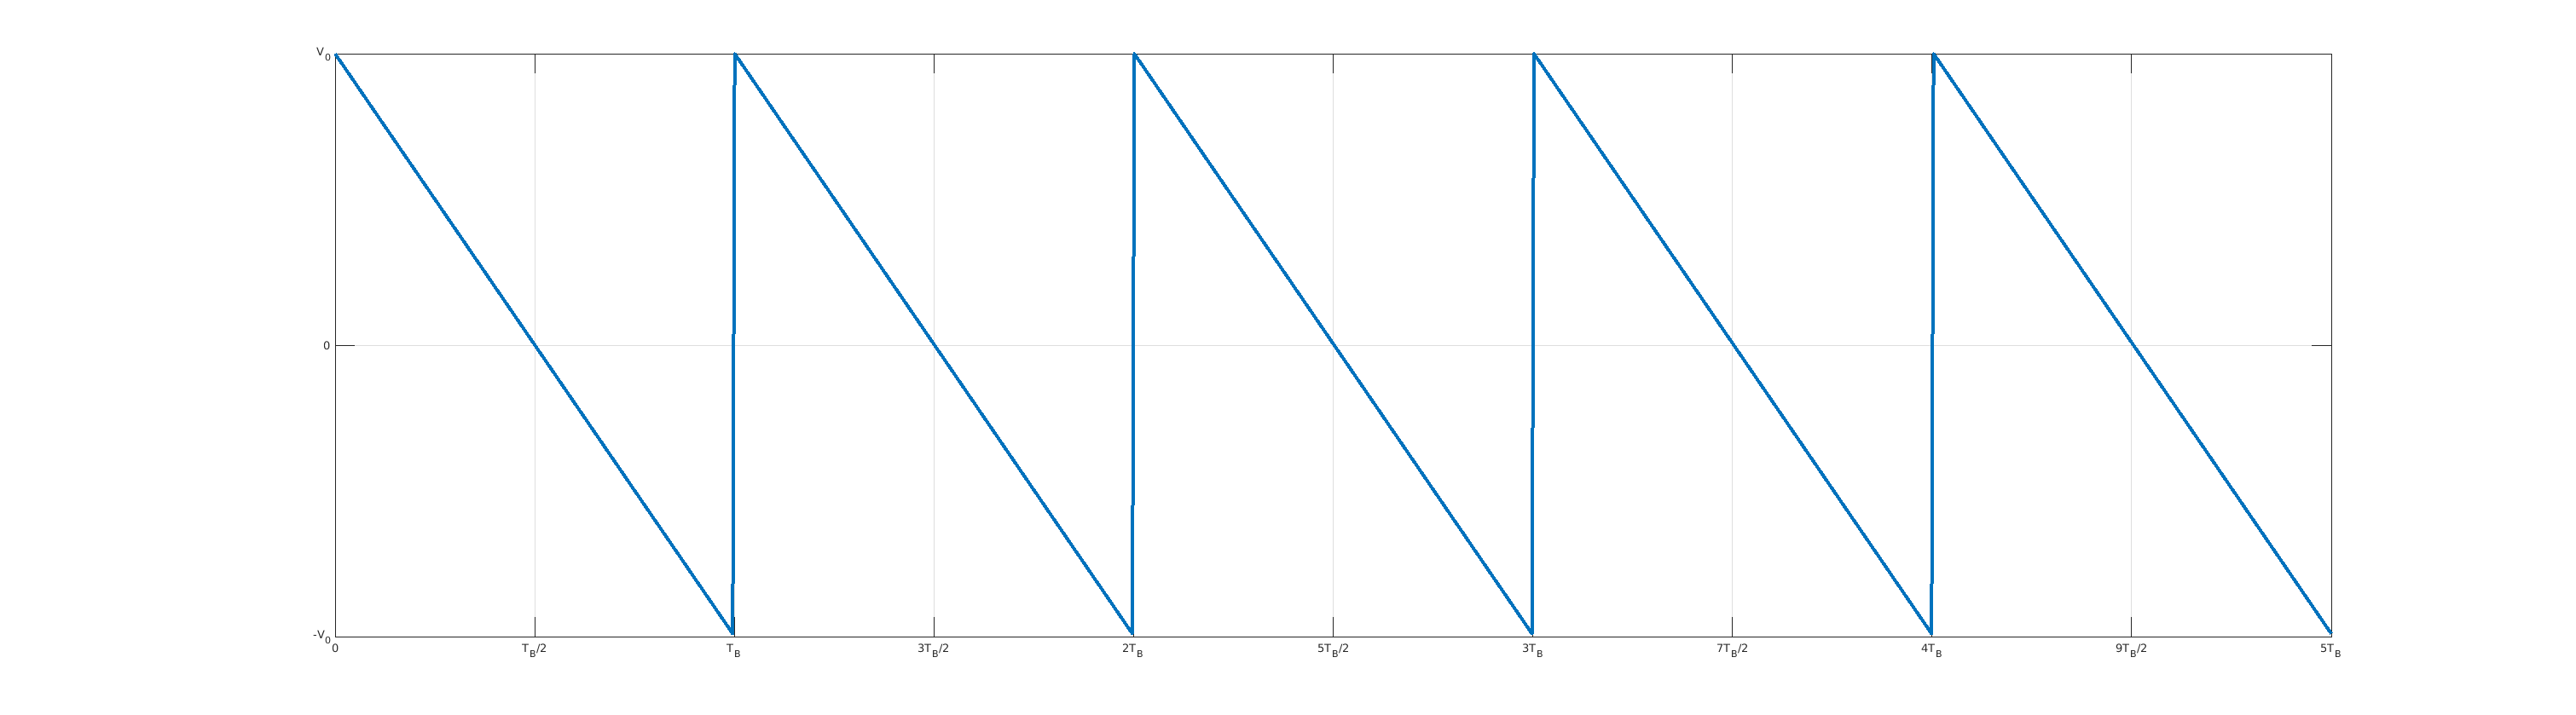
\includegraphics[width=\textwidth]{Figures/inputsignal.png}
\caption{Form of the signal coming out of the Telesto, used as the input to the circuit.}
\label{input}
\end{figure}

\begin{figure}[h!]
\centering
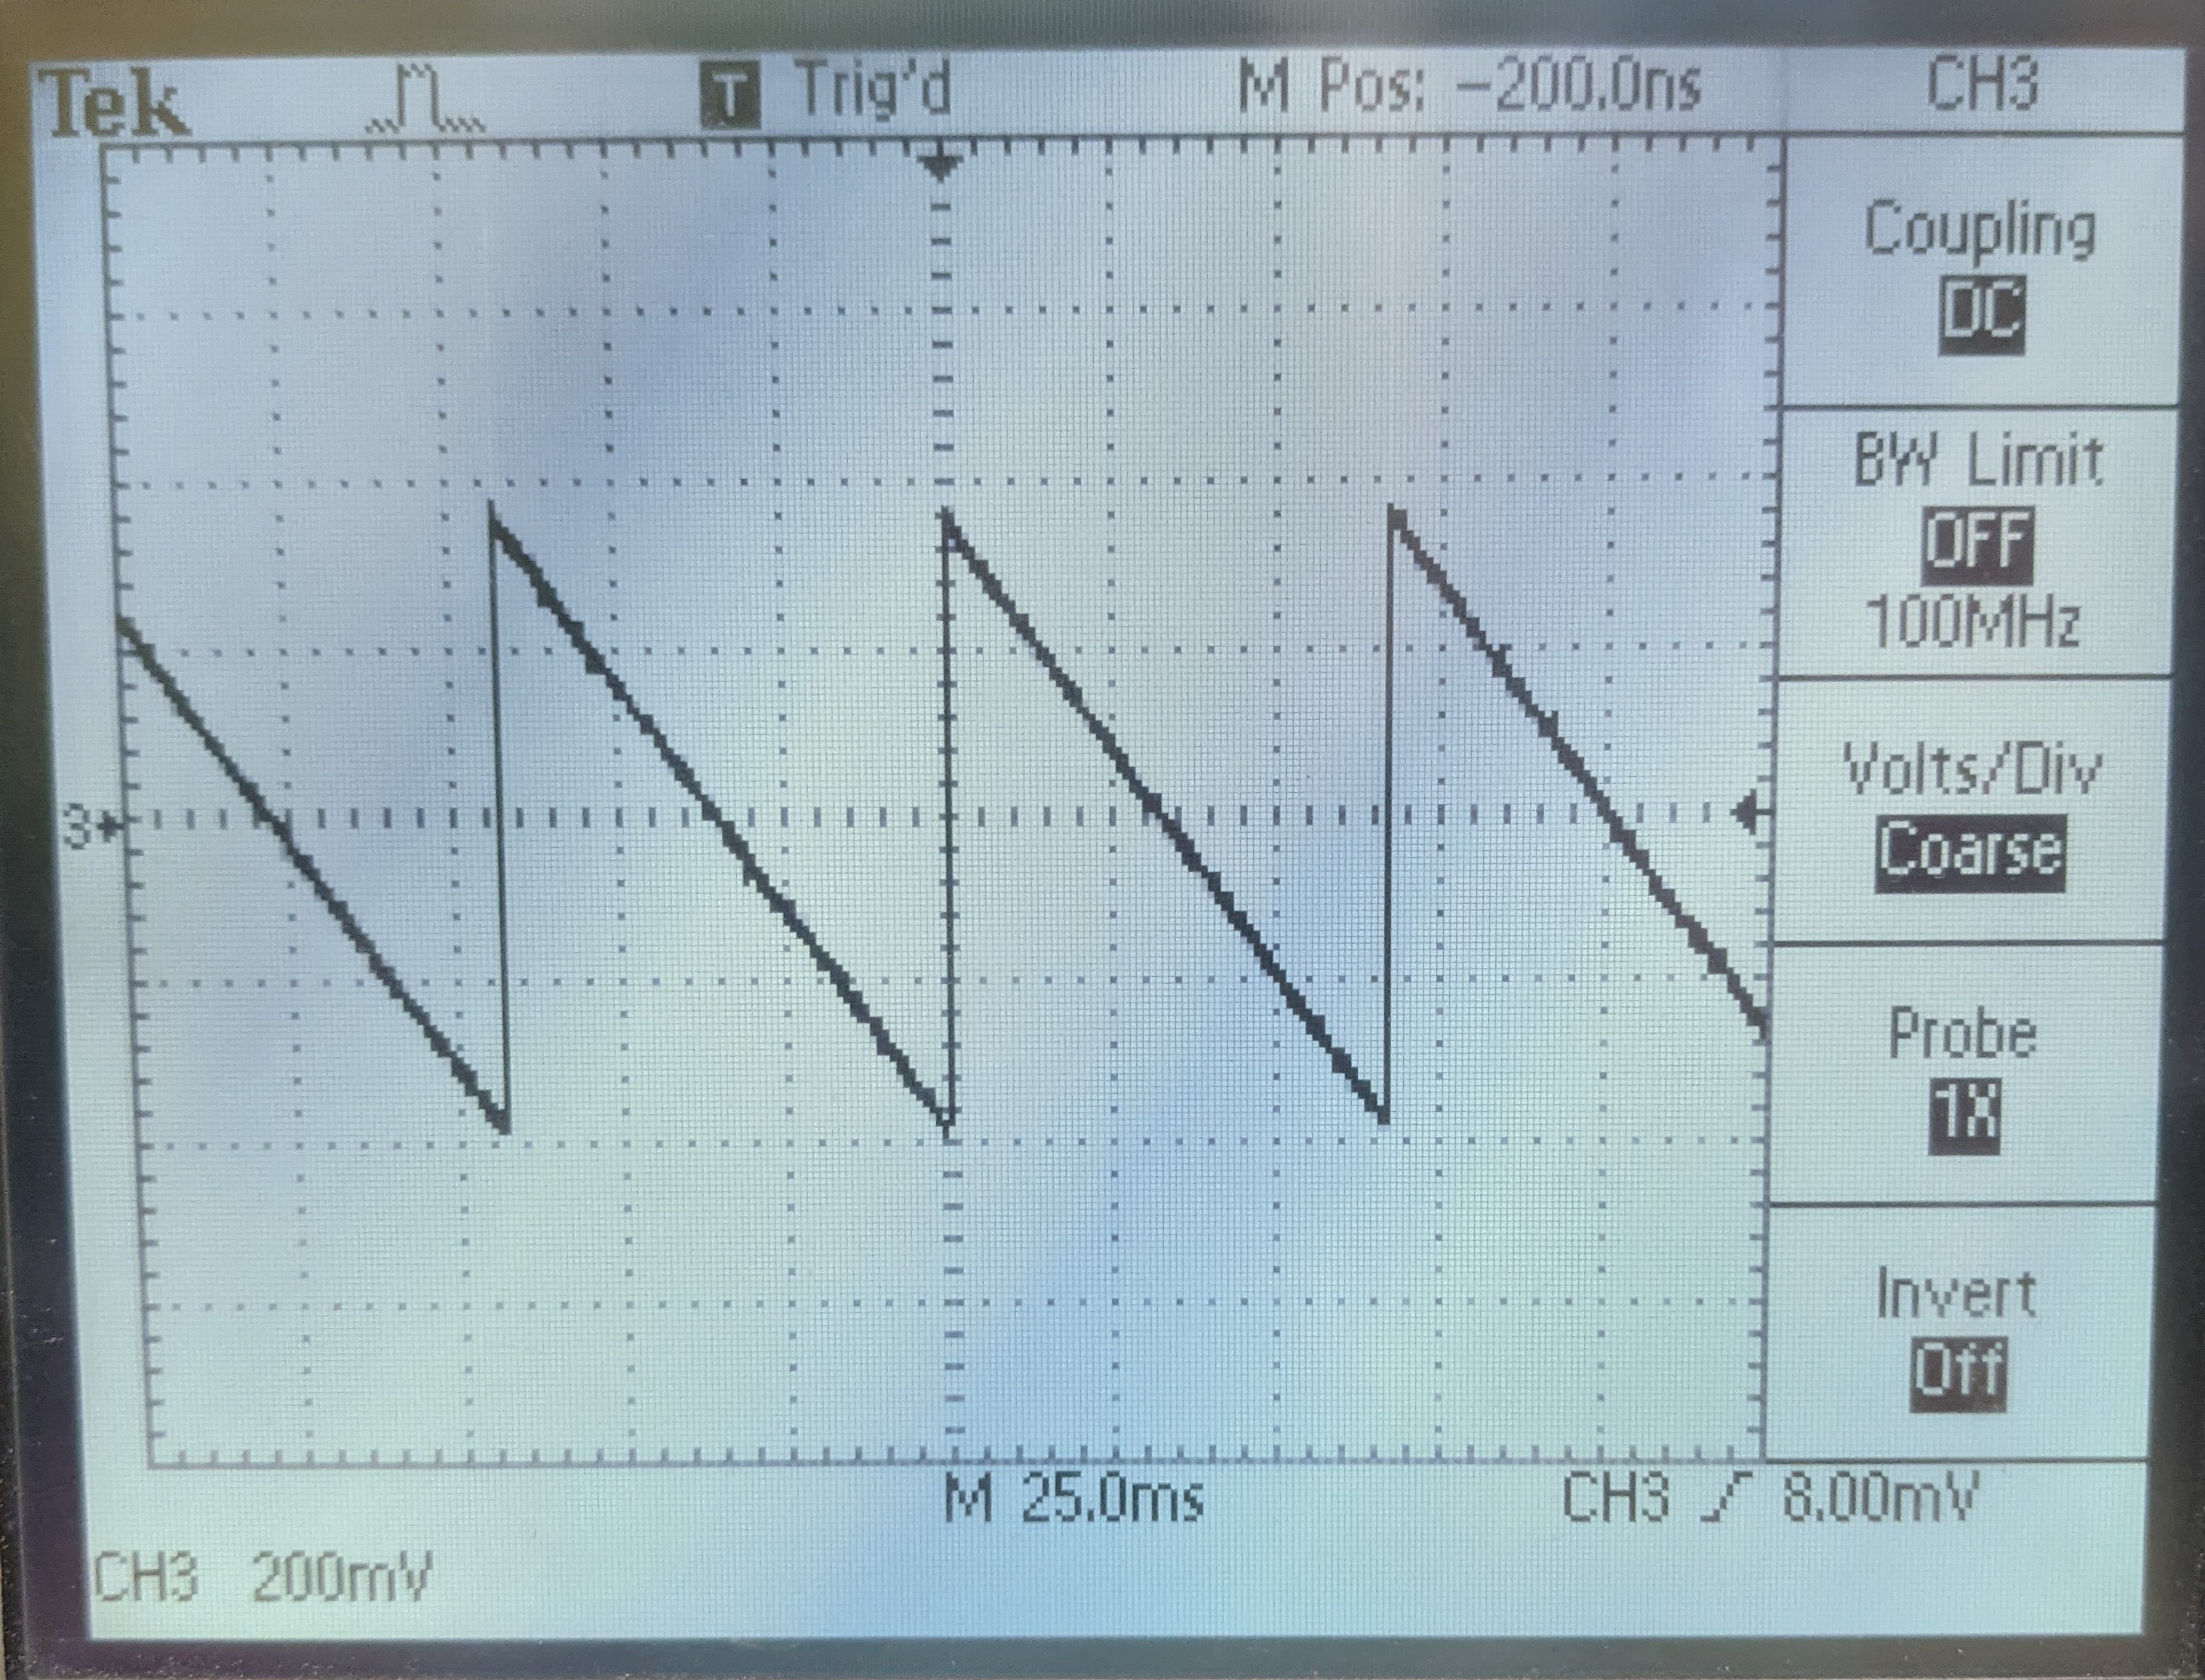
\includegraphics[width=.5\textwidth]{Figures/inputscope.jpg}
\caption{The signal coming out of the Telesto with $f_S=146$ kHz, $N=10000$ and $FOV=1$ mm.}
\label{inputscope}
\end{figure}


\begin{figure}
\centering
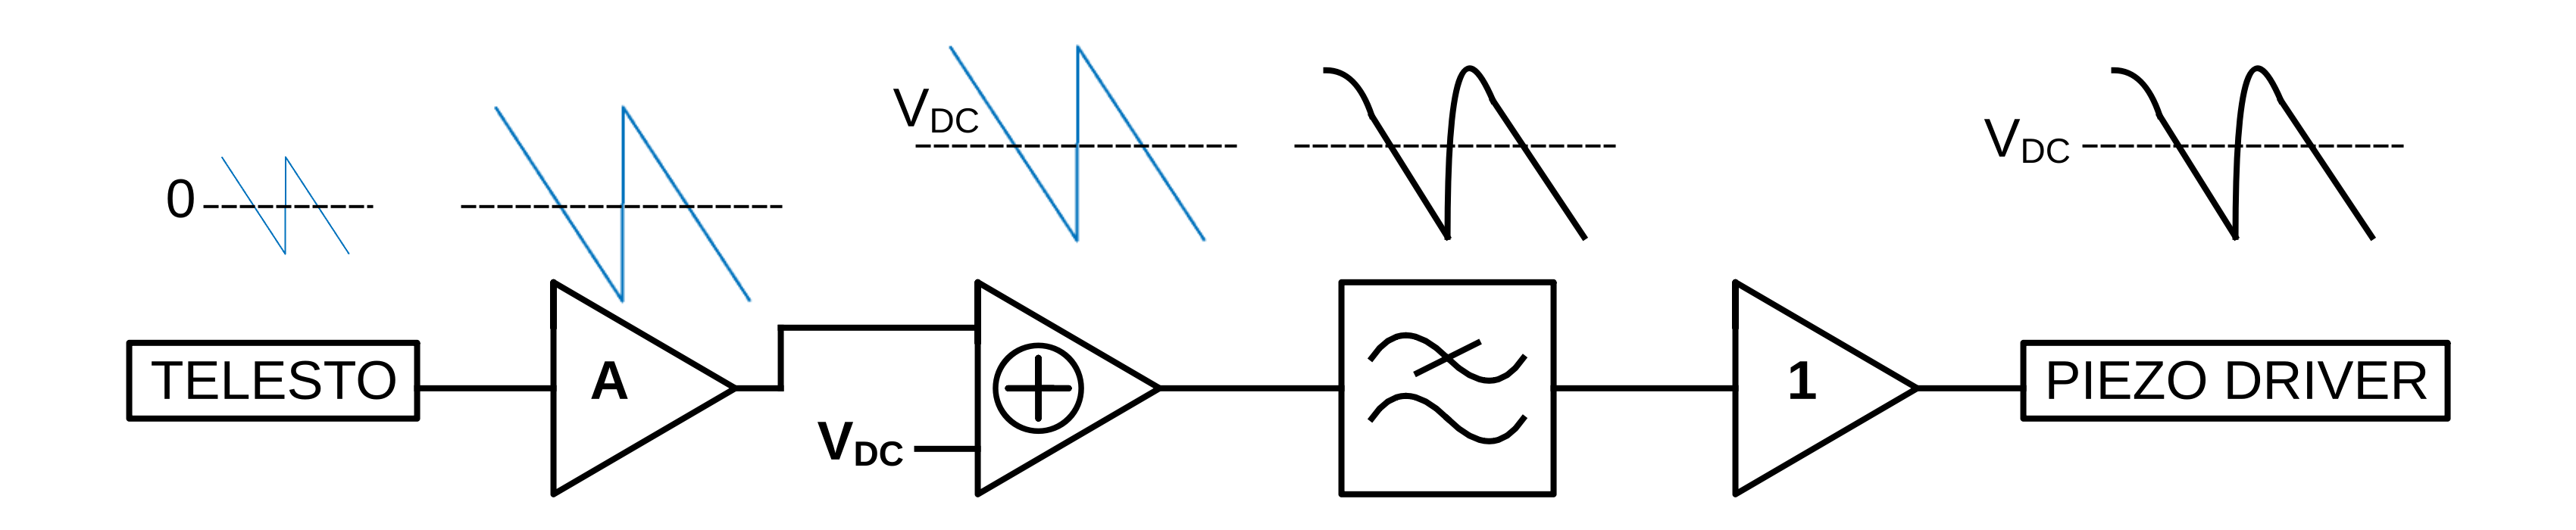
\includegraphics[width=\textwidth]{Figures/ProbeDriverBlock.png}
\caption{Block diagram for the scanning circuit, including the form of the signal after each block.}
\label{block}
\end{figure}



\begin{figure}
\centering
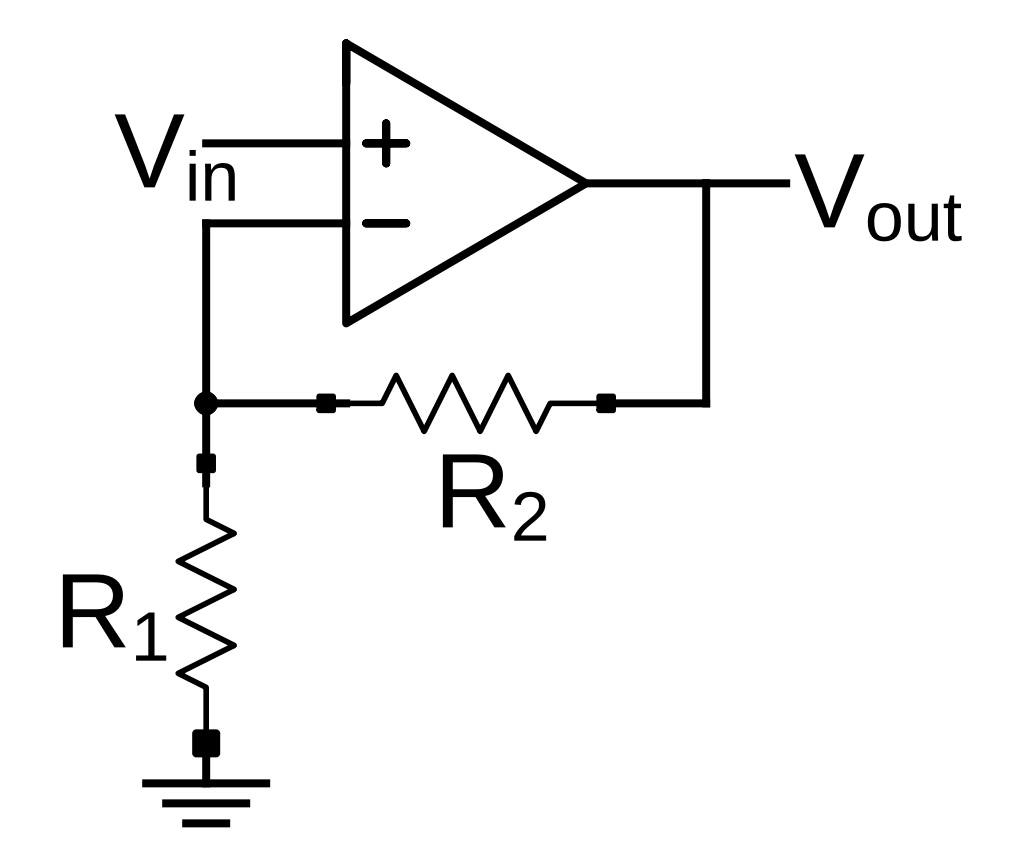
\includegraphics[width=.5\textwidth]{Figures/noninvamp.png}
\caption{Diagram of a non-inverting amplifier with gain $A= 1+ \frac{R_2}{R_1}$.}
\label{noninvamp}
\end{figure}



\begin{figure}
\centering
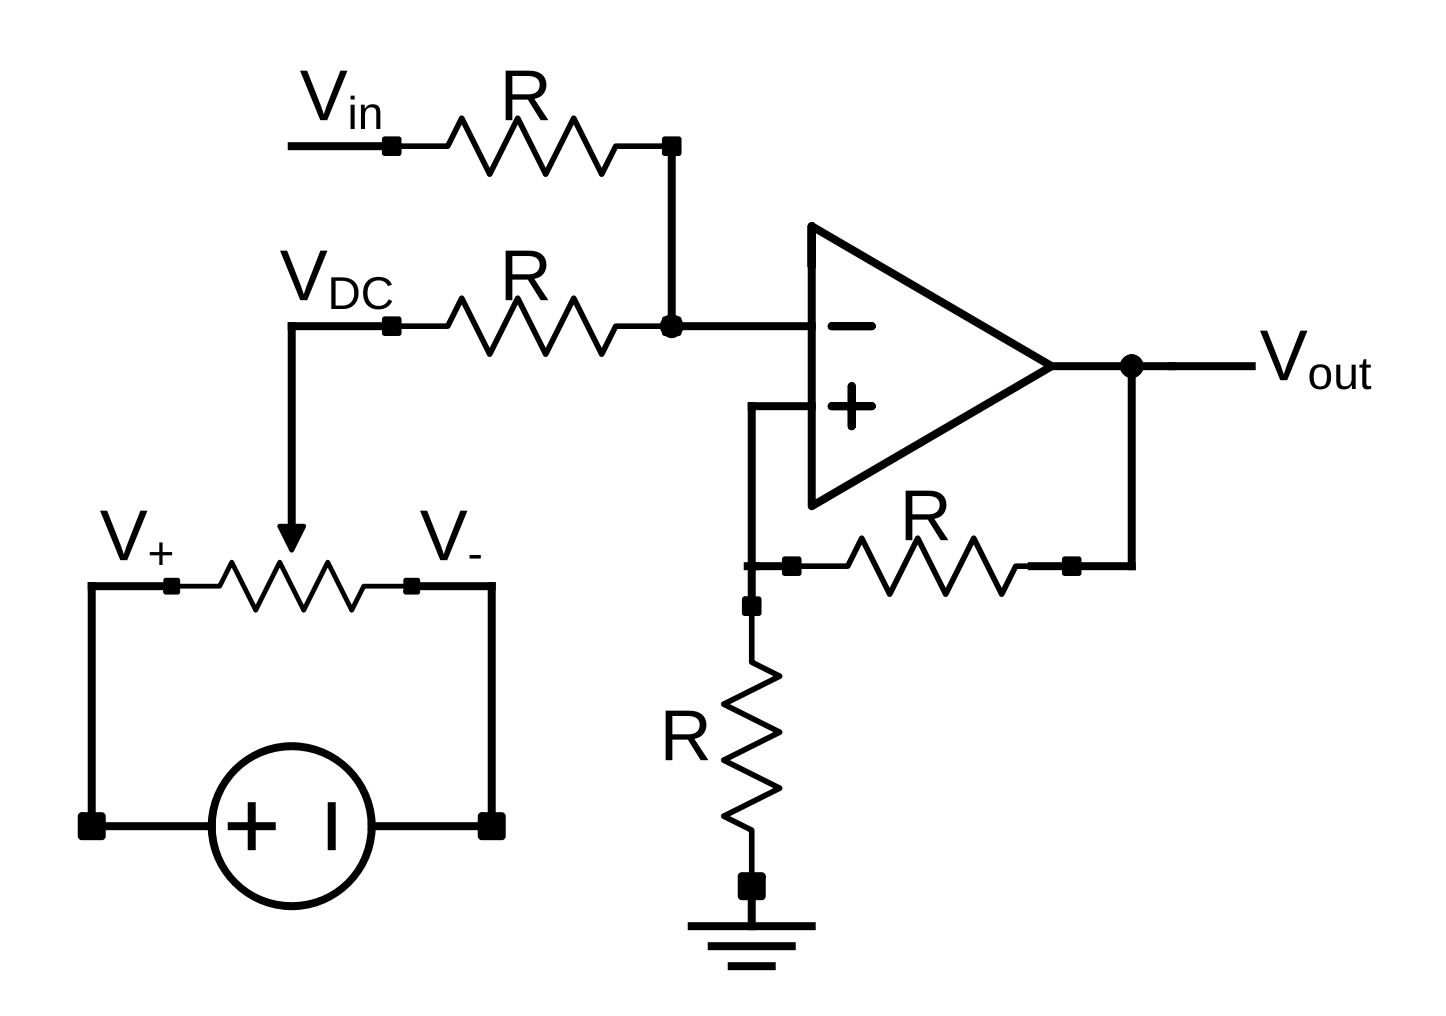
\includegraphics[width=.5\textwidth]{Figures/summer.png}
\caption{Diagram of a unity-gain summing amplifier with $V_{out} = V_{in}+V_{DC}$.}
\label{summer}
\end{figure}


\begin{figure}
\centering
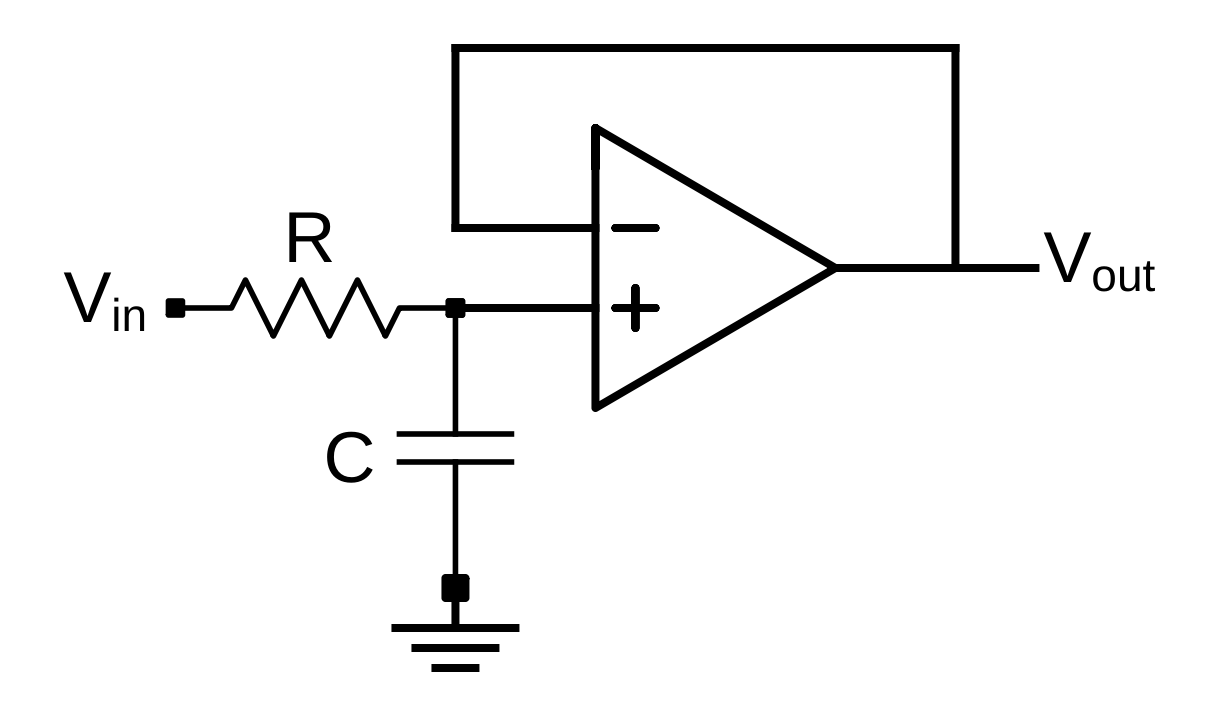
\includegraphics[width=.5\textwidth]{Figures/lpf.png}
\caption{Diagram of a first-order low-pass filter with cutoff frequency $f_C = \frac{1}{2\pi RC}$.}
\label{lpf}
\end{figure}


\begin{figure}
\centering
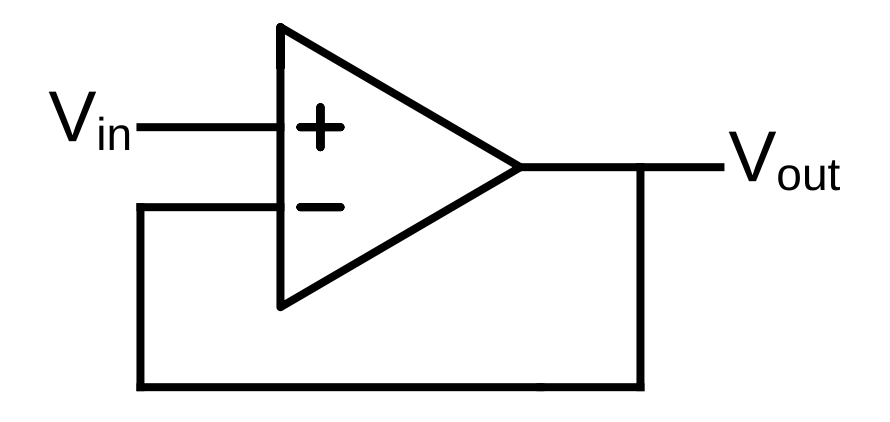
\includegraphics[width=.5\textwidth]{Figures/buffer.png}
\caption{Diagram of a unity-gain buffer.}
\label{buff}
\end{figure}



\begin{figure}
\centering
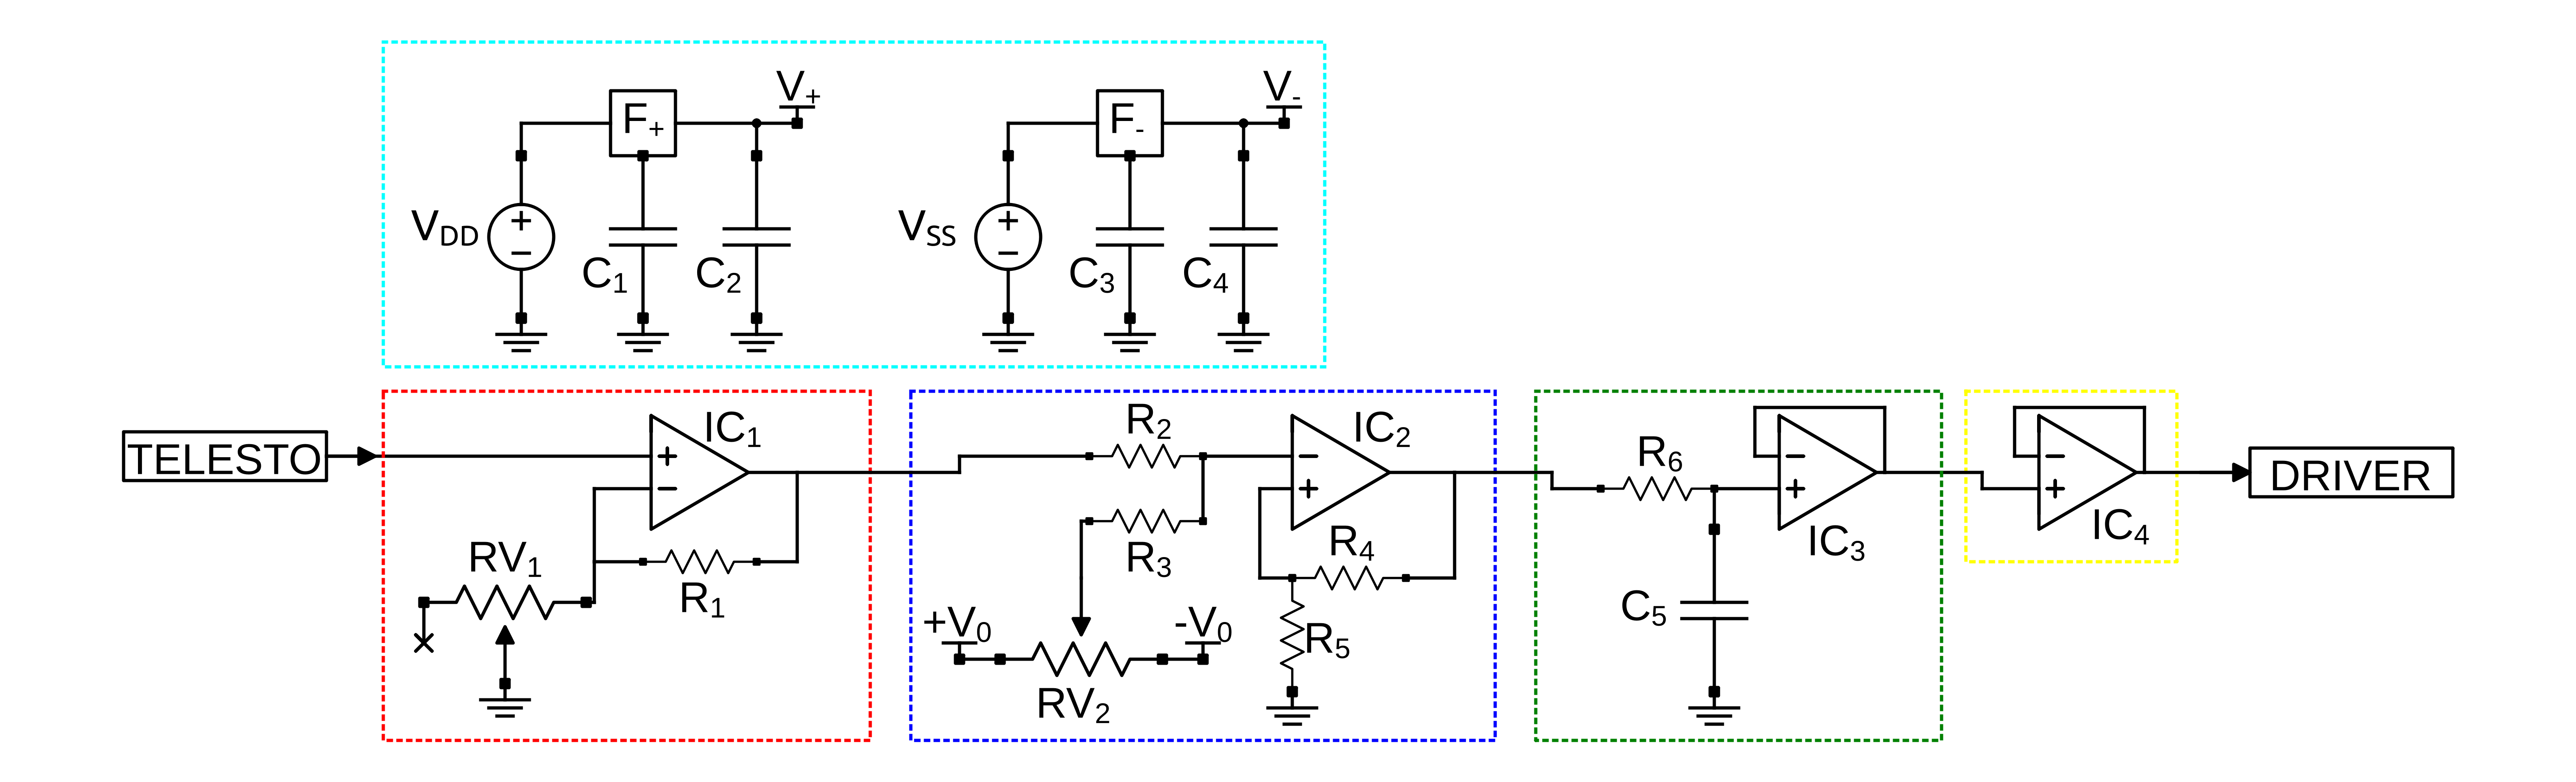
\includegraphics[width=\textwidth]{Figures/TotalSchem.png}
\caption{Schematic of the entire scanning circuit, with blocks in dotted squares. The amplifier, summing stage, LPF, buffer and power circuitry lie in red, blue, green, yellow and teal boxes, respectively.}
\label{schem}
\end{figure}

\begin{table}
	\centering
	\begin{tabular}{|c|c||c|c|}
	\hline
	PART LABEL & VALUE & PART LABEL & VALUE\\
	\hline \hline $R_{1-6}$ & 100 k$\Omega$ & $V_+$ & +9 V \\
	\hline $RV_1$ & 50 k$\Omega$ & $V_-$ & -9 V\\
	\hline $RV_2$ & 500 k$\Omega$ & $V_{DD}$ & +15 V\\
	\hline $C_{1,3}$ & 0.1 $\mu$F & $V_{SS}$ & -15 V\\
	\hline $C_{2,4}$ & 0.1 $\mu$F $||$ 0.47 $\mu$F & $F_+$ & BA90DD0WT-ND\\
	\hline $C_5$ & 0.1 $\mu$F & $F_-$ & 2368-NTE1967-ND\\ 
	\hline $IC_{1-4}$ &  LM741CN & Power Supply & TDK-Lambda KMD15-1515 \\ 
	\hline
	\end{tabular}
	\caption{Table of values used in the implementation of the scanning circuit. The decoupling capacitors $C_{2}$ and $C_4$ are each implemented via two capacitors in parallel forming a total capacitance of 0.57 $\mu$F each.}
	\label{materials}
\end{table}


\begin{figure}
\centering
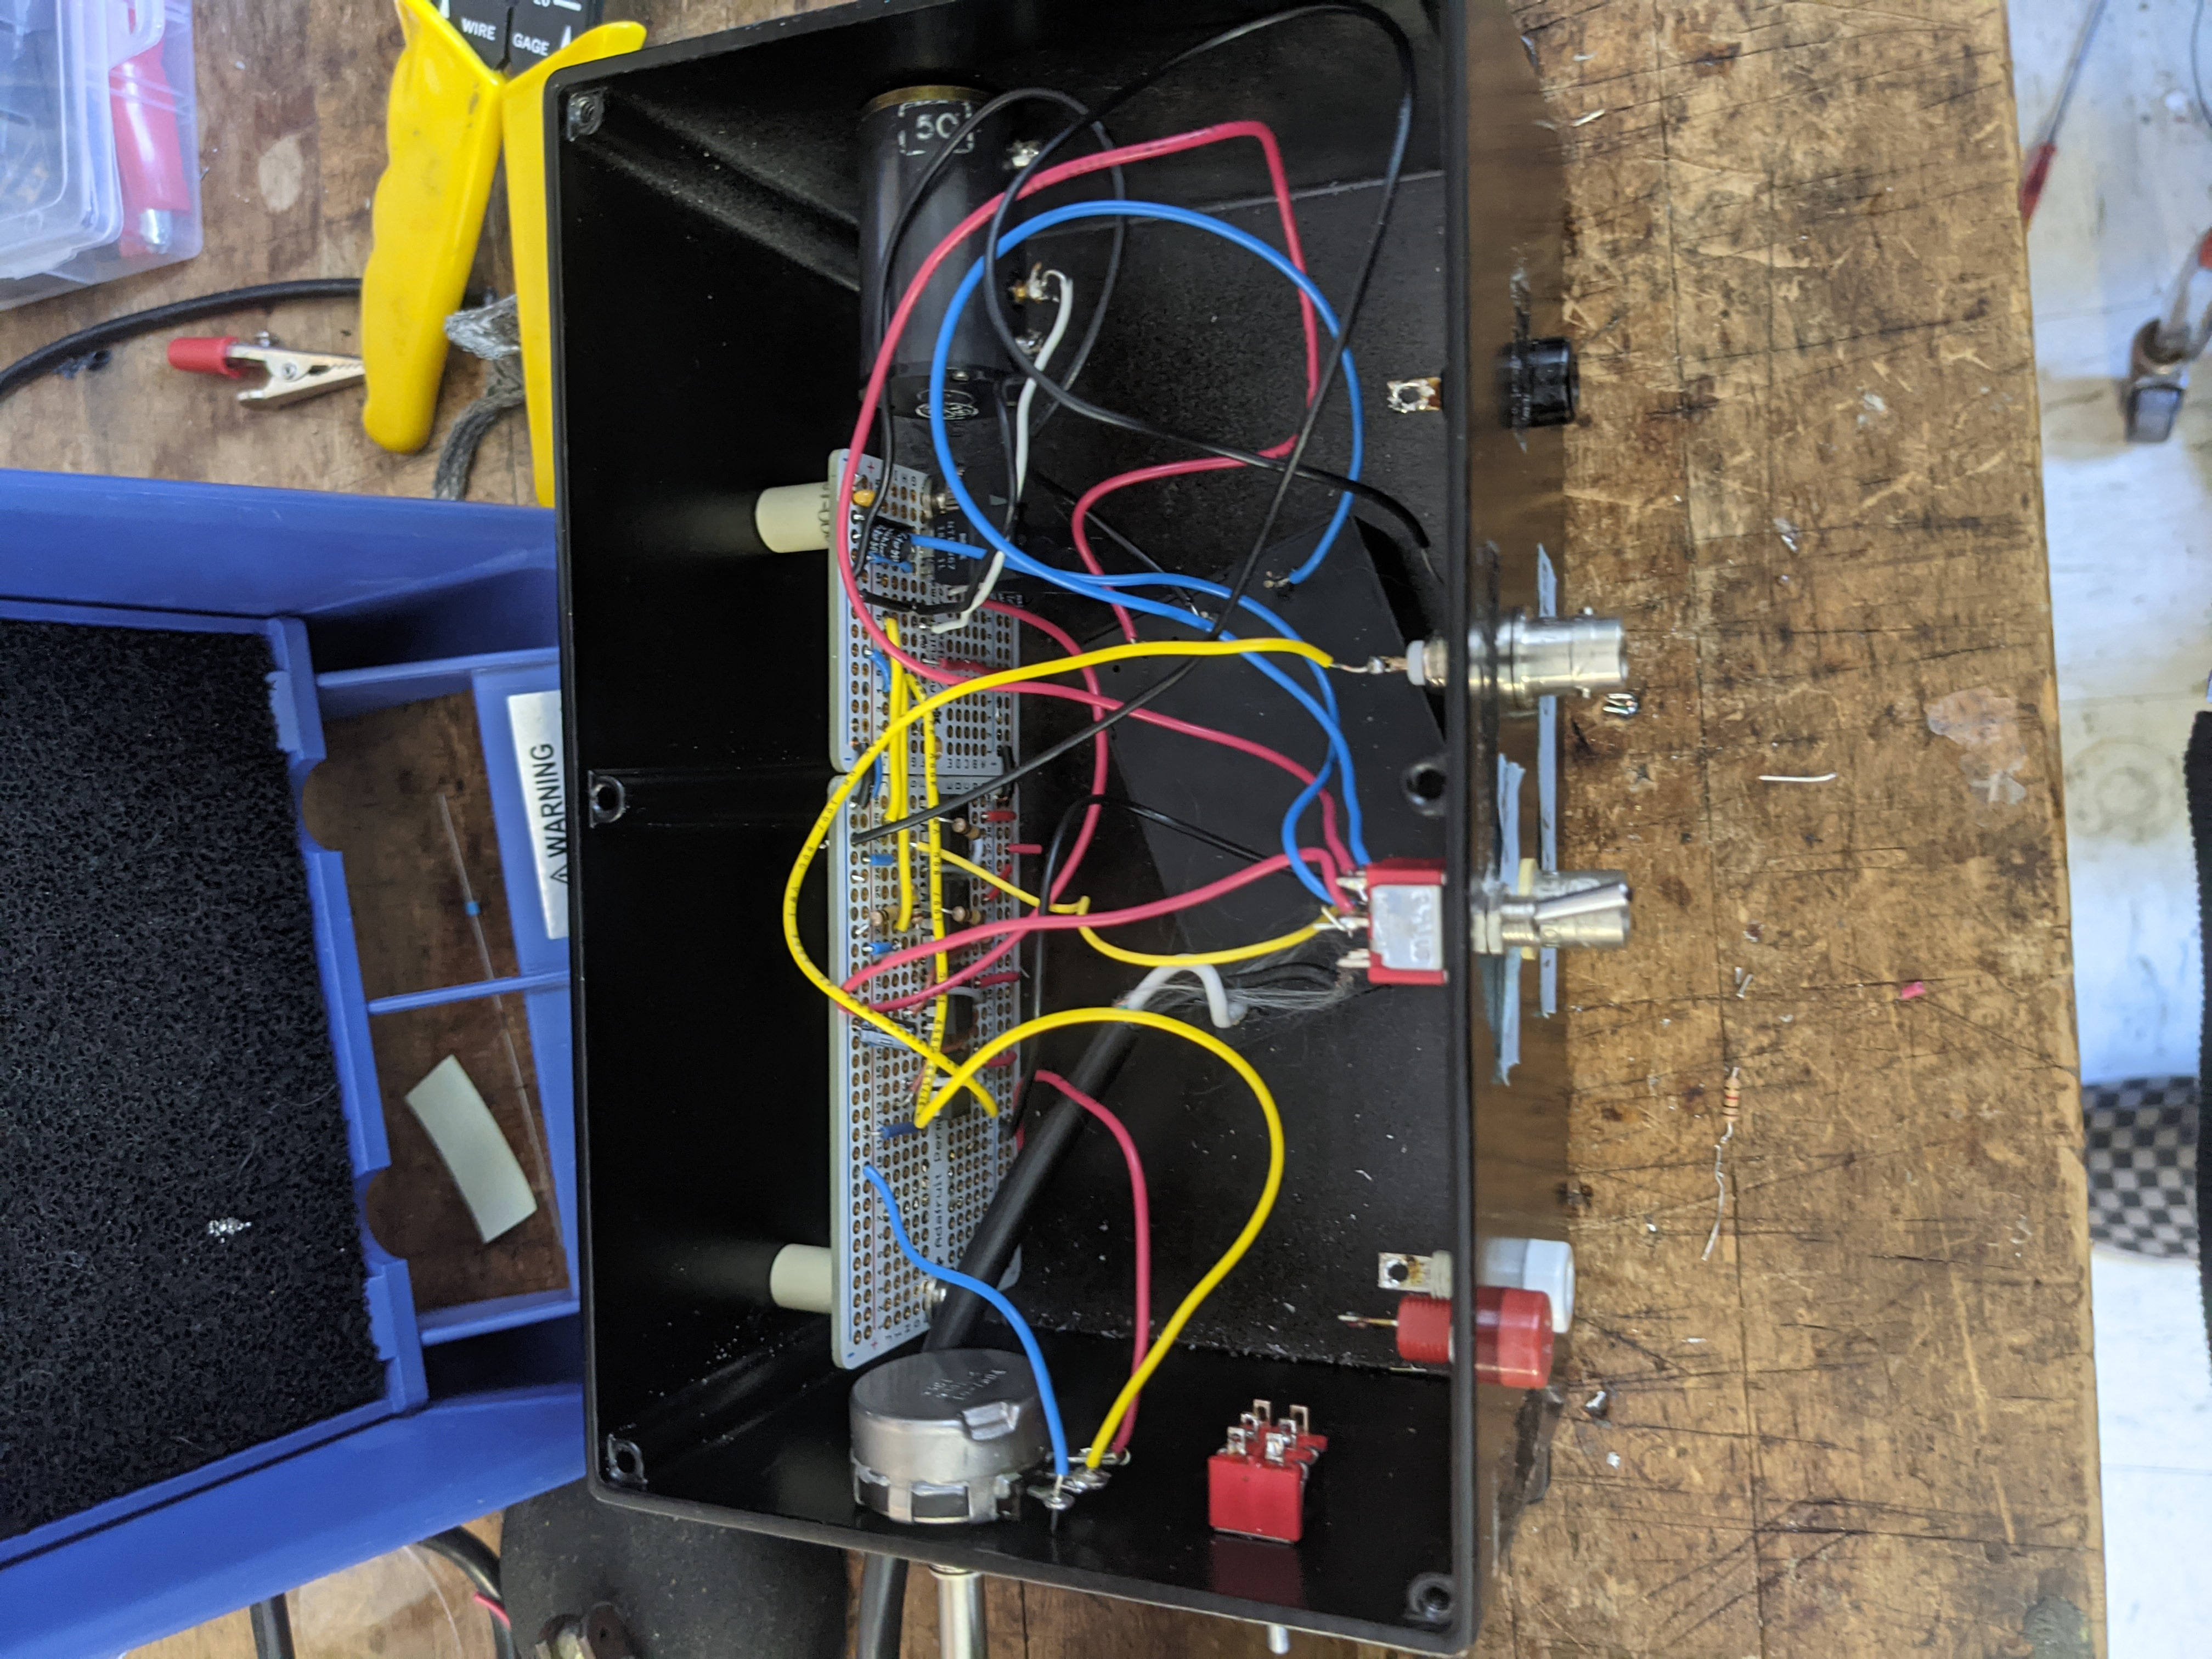
\includegraphics[width=\textwidth,angle=-90,origin=c]{Figures/InsideCircuit.jpg}
\caption{Interior of the box containing the circuit, showing the breadboards attached to the back side of the box. The power supply lies on the bottom, the DC offset potentiometer is on the left and the gain potentiometer is on the right. The ON/OFF switch is at the front.}
\label{inside}
\end{figure}

\begin{figure}
\centering
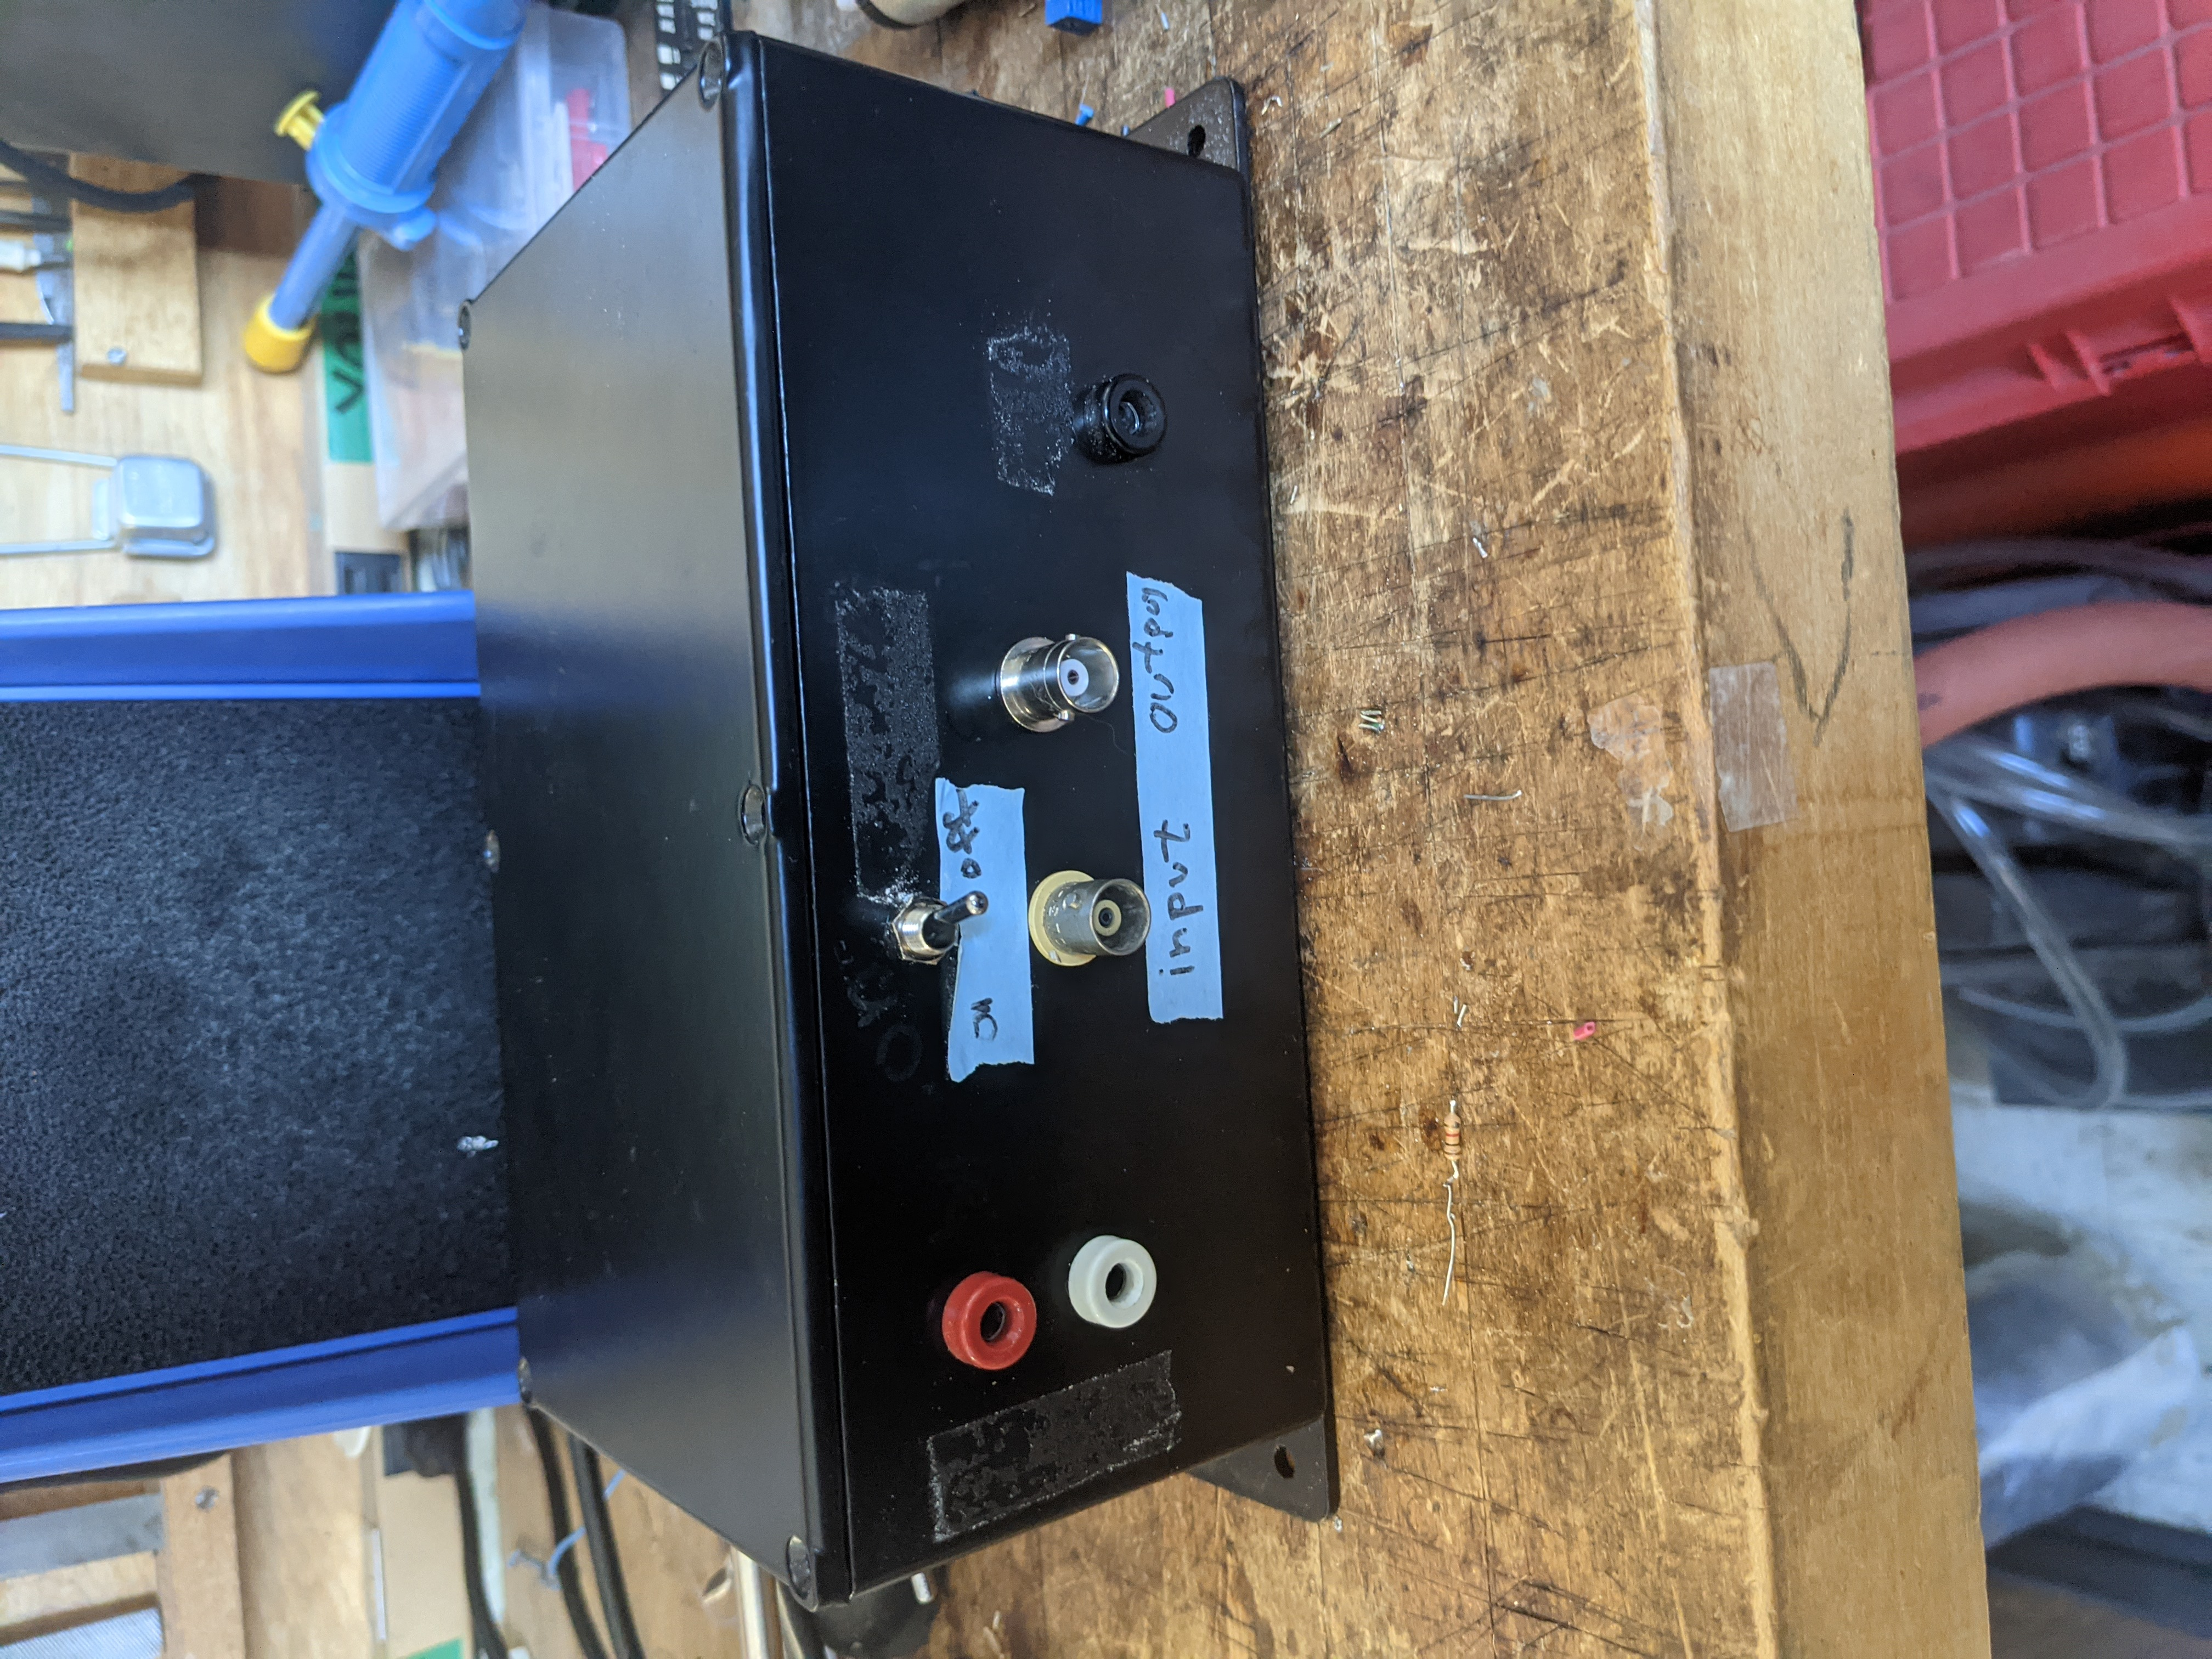
\includegraphics[width=\textwidth,angle=-90,origin=c]{Figures/OutsideCircuit.jpg}
\caption{The exterior of the scanning circuit, in a grounded box. There are input and output BNC connectors, an ON/OFF switch, a DC offset control potentiometer on the left and a gain control potentiometer on the right.}
\label{outside}
\end{figure}



\begin{figure}
\centering
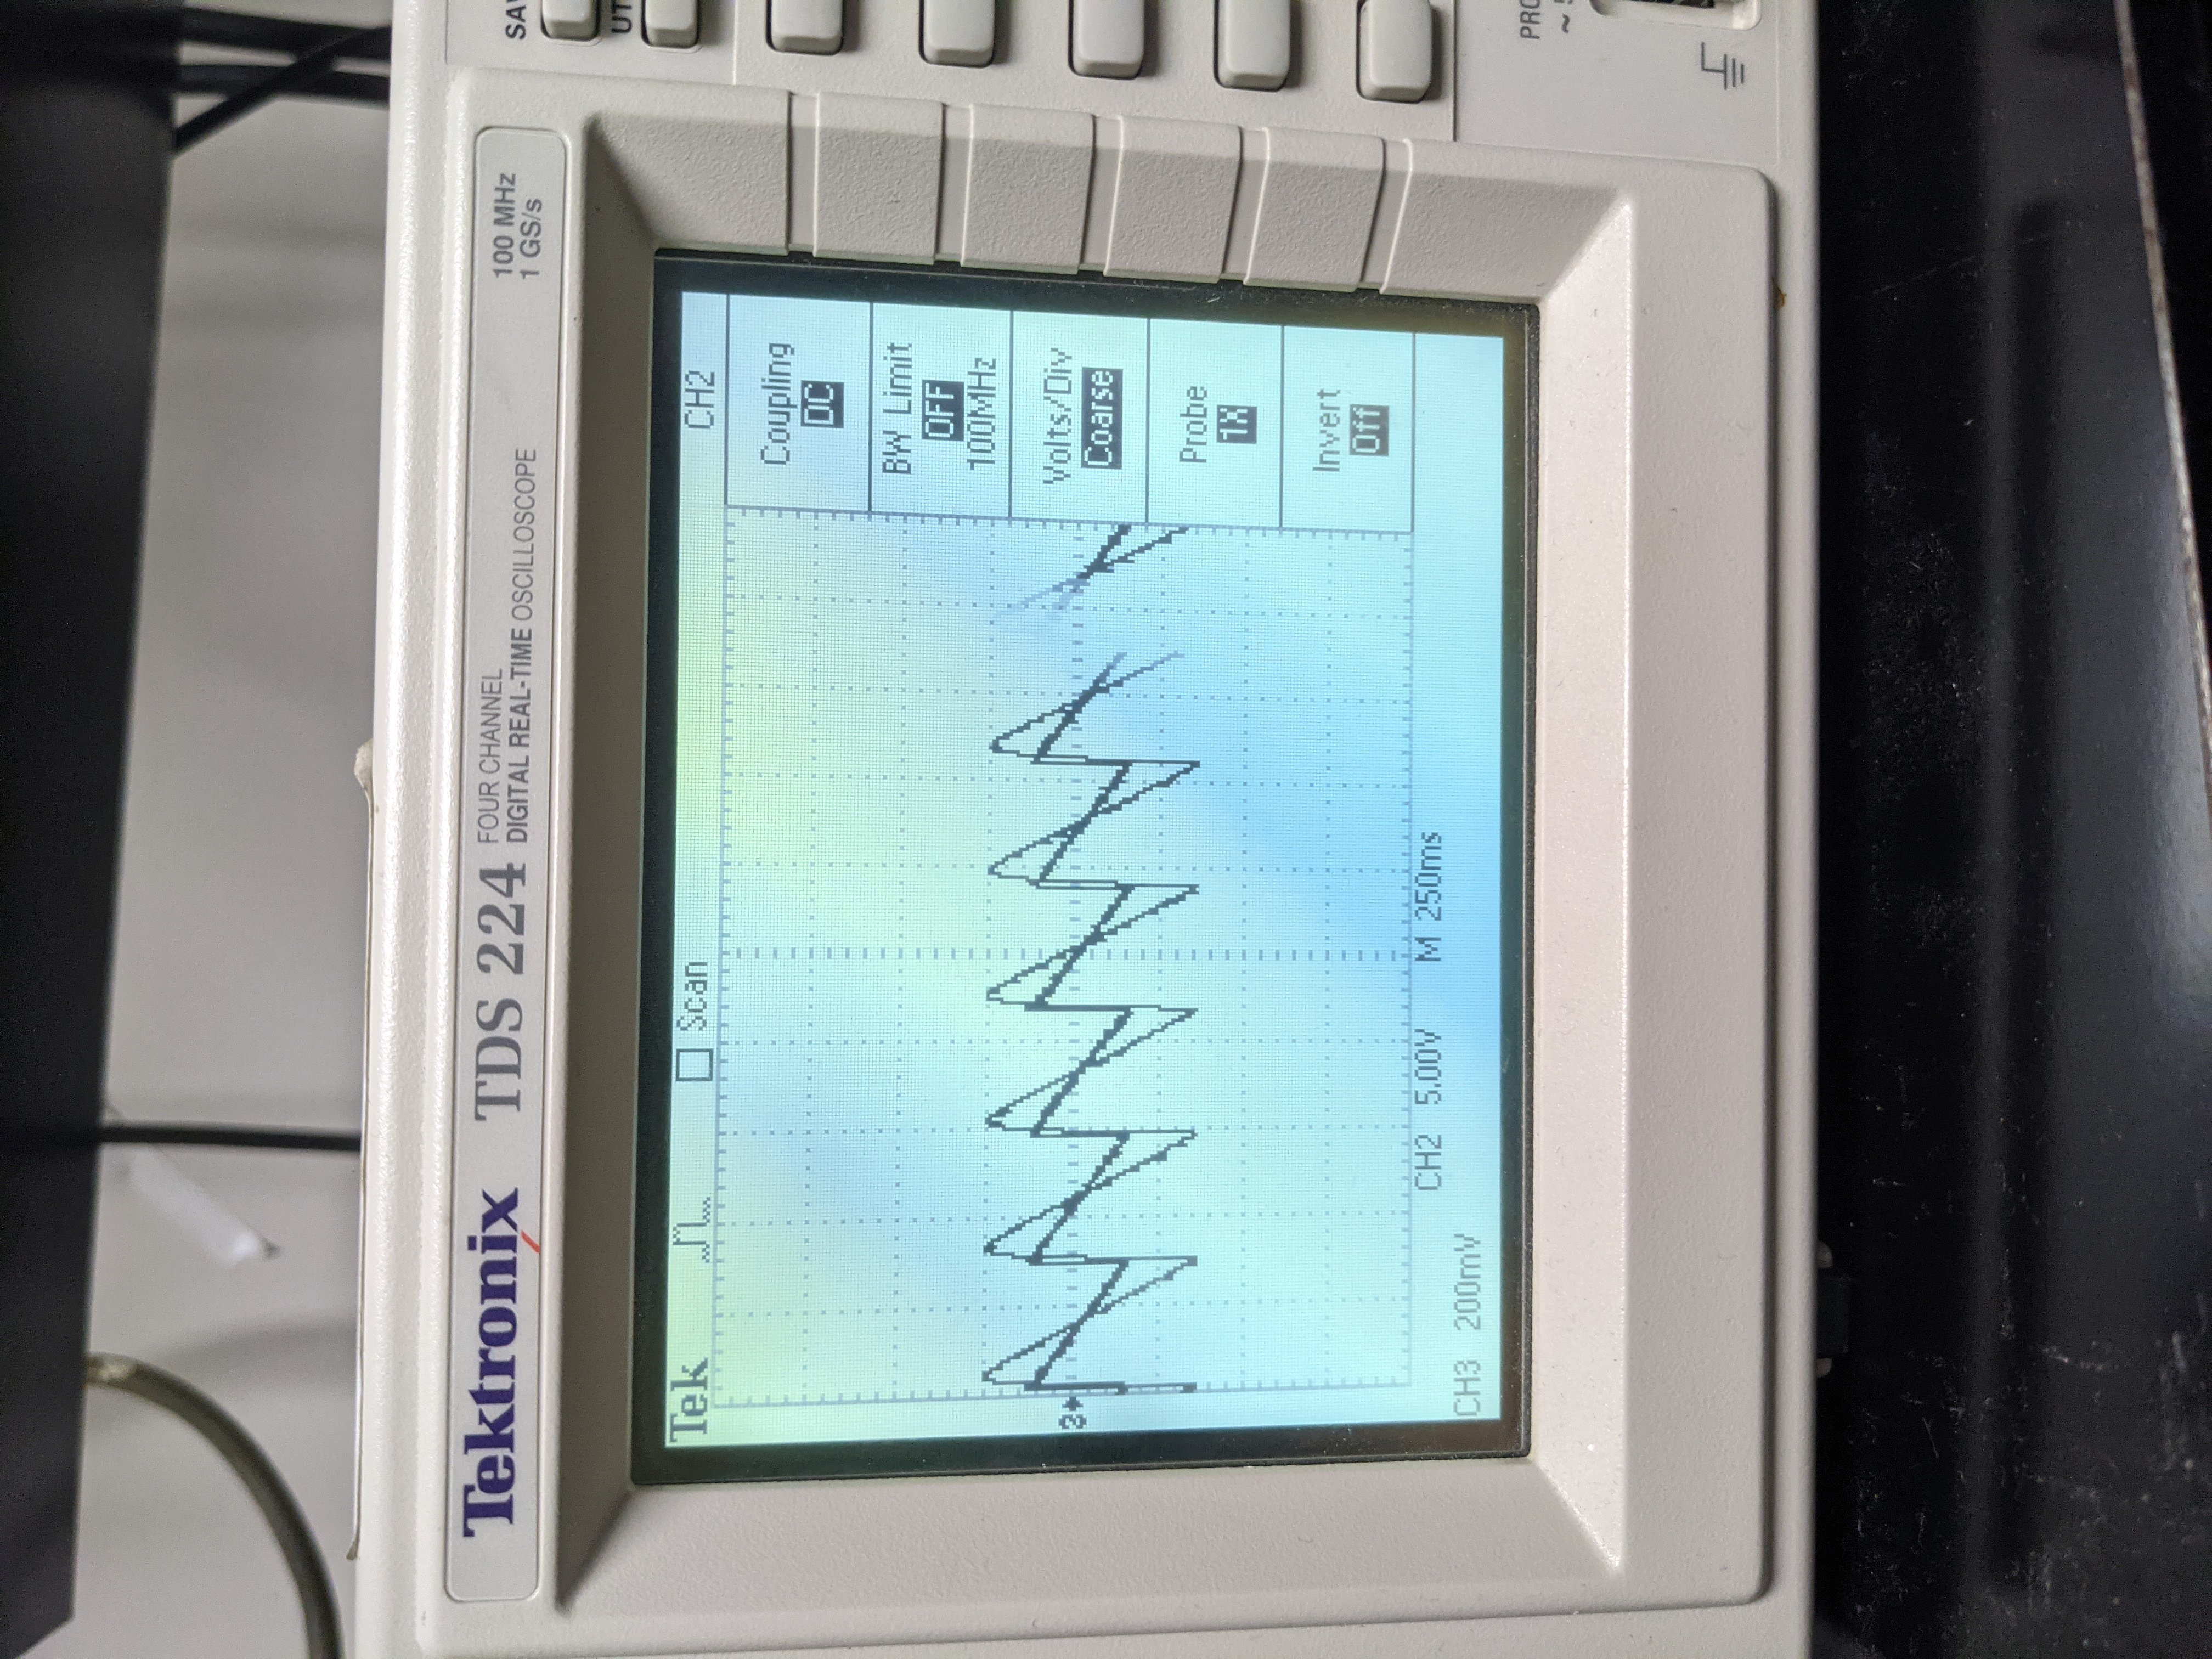
\includegraphics[width=\textwidth,angle=-90,origin=c]{Figures/overlayscope.jpg}
\caption{Input (CH3) and output (CH2) of the circuit with DC offset ~0 and gain ~62.5. Note the time scale is 250 ms/div, the input scale is 200 mV/div and the output scale is 5V/div.}
\label{samplenormal}
\end{figure}

\begin{figure}
\centering
\includegraphics[width=\textwidth,angle=-90,origin=c]{Figures/offsetscope.jpg}
\caption{Input (CH3) and output (CH2) of the circuit with DC offset ~6 V and gain ~25. Note the time scale is 250 ms/div, the input scale is 200 mV/div and the output scale is 5V/div. This shows that the circuit can be controlled in offset and gain as desired.}
\label{sampleoffset}
\end{figure}


\begin{figure}
\centering
\includegraphics[width=\textwidth,angle=-90,origin=c]{Figures/saturatedscope.jpg}
\caption{Input (CH3) and output (CH2) of the circuit with very large gain. The voltage is seen to saturate at $\pm 8.5$ V, a bit below the rail voltages. We want this behavior, as it means the voltage will never surpass the input voltage range of the piezo driver. Note the time scale is 250 ms/div, the input scale is 250 mV/div and the output scale is 5V/div.}
\label{samplesaturated}
\end{figure}


\end{document}
